\documentclass{beamer}
\usetheme{Dresden}
\usepackage[spanish]{babel}
\usepackage[utf8]{inputenc}

\begin{document}
\title{Ciclo completo de CI/CD con Dagger y Kubernetes}
\subtitle{Grado en Ingeniería Informática \\
    Universidad de Santiago de Compostela}
\author{Autor: Daniel Vieites Torres}
\institute{Tutor: Juan Carlos Pichel Campos \\ Co-tutor: Francisco Maseda Muiño}
\date{\today}

\begin{frame}
    \titlepage
\end{frame}

\begin{frame}
    \frametitle{Tabla de contenidos}\tableofcontents
\end{frame}

\section{Objetivos}
\subsection{El problema}
\begin{frame}
    \frametitle{¿Cuál es el problema?}
    \begin{columns}
        \begin{column}{0.45\textwidth}
            \begin{itemize}
                \item<1-> Aplicaciones con un gran volumen de tecnologías.
                \item<2-> Gran complejidad.
                \item<3-> Coste de mantenimiento elevado.
            \end{itemize}
        \end{column}
        \begin{column}{0.55\textwidth}
            \begin{figure}
                \includegraphics<1>[height=4.8cm]{figuras/Gitlab}
                \only<1>{\caption{Arquitectura de GitLab.}}
                \includegraphics<2>[scale=0.33]{figuras/complejidad}
                \includegraphics<3>[scale=0.15]{figuras/costes-mantenimiento}
                \only<3>{\caption{Imagen generada con IA.}}
            \end{figure}
        \end{column}
    \end{columns}
\end{frame}

\subsection{La solución}

\begin{frame}
    \frametitle{¿Qué se propone?}
    \begin{center}
        {\it Dagger} para gestionar CI/CD.
    \end{center}
    \begin{figure}
        
\includegraphics[scale=1.2]{figuras/Dagger_logo}
    \end{figure}
    % ¿Qué es Dagger?
    % ¿Cómo de complejo es?
    %   - curva de aprendizaje
    % ¿Facilita el desarrollo?
    %   - comparado con tecnologías tradicionales
    % ¿Disminuye los costes de soporte?
    %   - del que se habló antes
    % ¿Permite la independencia de plataforma?
\end{frame}

\begin{frame}
    \frametitle{CI/CD}
    \begin{figure}
        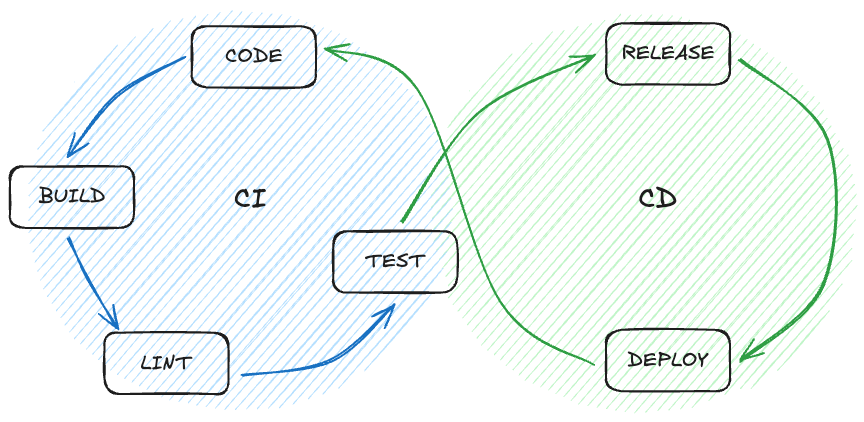
\includegraphics[scale=0.35]{figuras/ci_cd}
        \caption{Ciclo de CI/CD de este TFG.}
    \end{figure}
\end{frame}

\begin{frame}
    \frametitle{Dagger}
    \begin{columns}
        \begin{column}{0.45\textwidth}
            \begin{itemize}
                \item<1-> SDK de creación de \textit{pipelines} de CI/CD.
                \item<2-> Múltiples lenguajes.
                      % Sin necesidad de entrelazar scripts de manera
                      % compleja. Uso del mismo lenguaje de programación.
                      % Más abstracción.
                \item<3-> Módulos.
                \item<4-> {\it Runtime} de OCI.
                      % Permite ejecución local
                \item<5-> Uso de caché.
            \end{itemize}
        \end{column}
        \begin{column}{0.55\textwidth}
            \begin{figure}
                \includegraphics<1>[scale=0.2]{figuras/dagger}
                \includegraphics<2>[scale=0.25]{figuras/languages}
                \includegraphics<3>[scale=0.4]{figuras/daggerverse}
                \includegraphics<4>[scale=0.4]{figuras/docker}
                \includegraphics<5>[scale=0.1]{figuras/cache}
                \only<5>{\caption{Imagen generada con IA.}}
            \end{figure}
        \end{column}
    \end{columns}
\end{frame}

\section{Organización}
\begin{frame}
    \frametitle{Organización de GitHub}
    \begin{figure}
        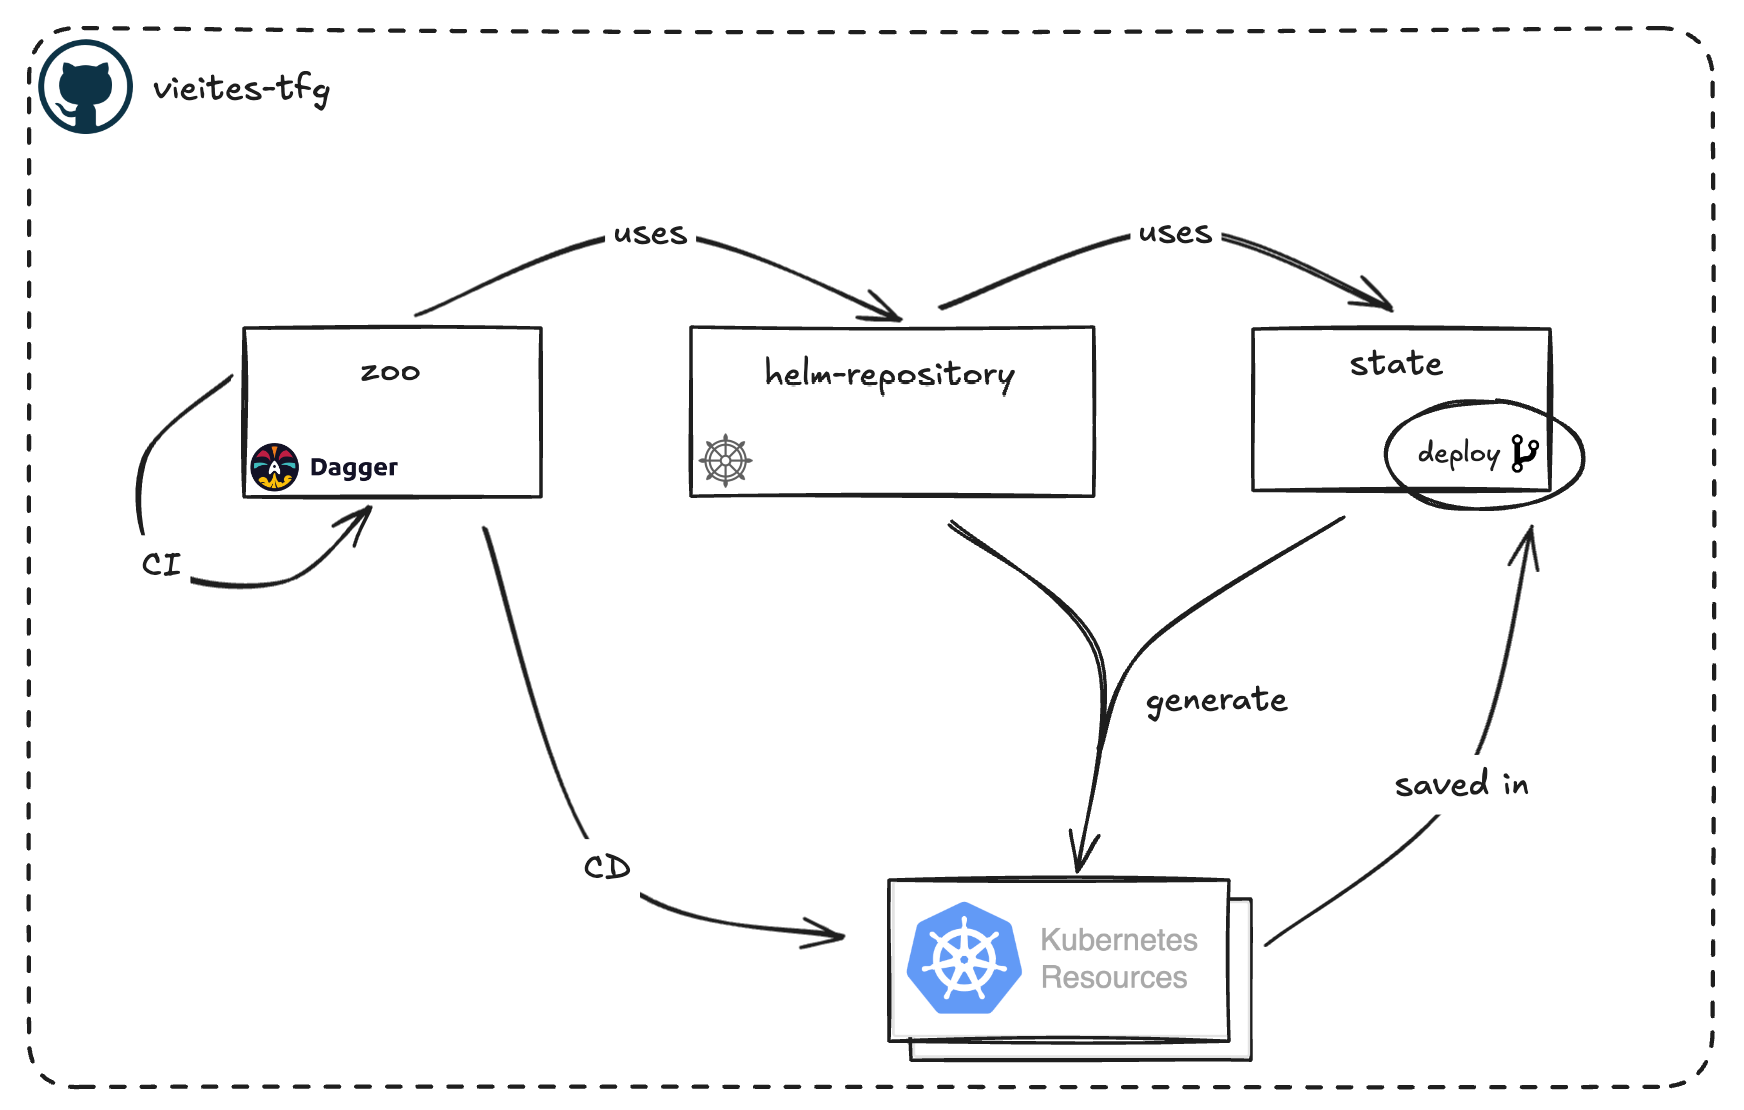
\includegraphics[scale=0.28]{figuras/vieites-tfg}
    \end{figure}
\end{frame}

\section{CI}
\subsection{App}
\begin{frame}
    \frametitle{Zoo}
    \begin{figure}
        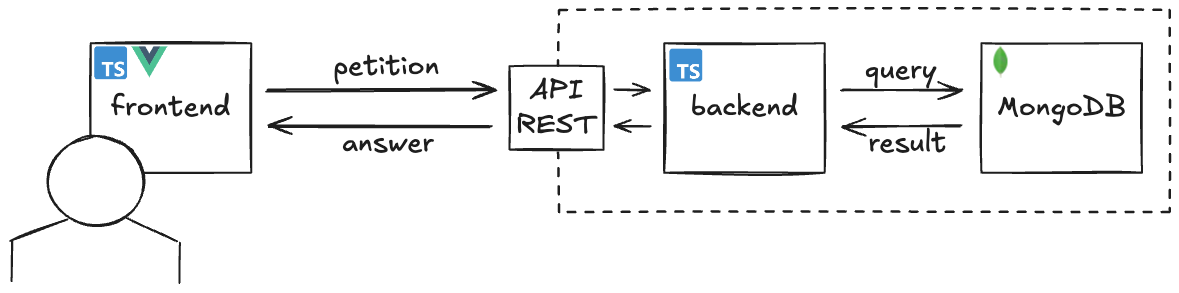
\includegraphics[scale=0.25]{figuras/app}
        \caption{Elementos de la aplicación.}
    \end{figure}
\end{frame}

\subsection{CI con Dagger}
\begin{frame}
    \frametitle{Tengo que explicar CI}
\end{frame}

\section{CD}
\subsection{Estructura de despliegue}
\begin{frame}
    \frametitle{helm-repository}
    \begin{figure}
        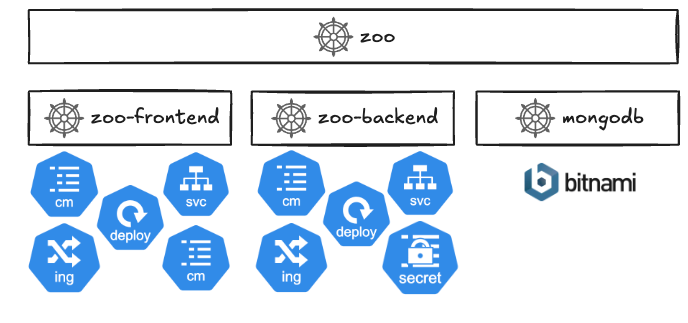
\includegraphics[scale=0.4]{figuras/helm-repository}
        \caption{Estructura de despliegue de la aplicación.}
    \end{figure}
\end{frame}

\begin{frame}
    \frametitle{state}
    \begin{figure}
        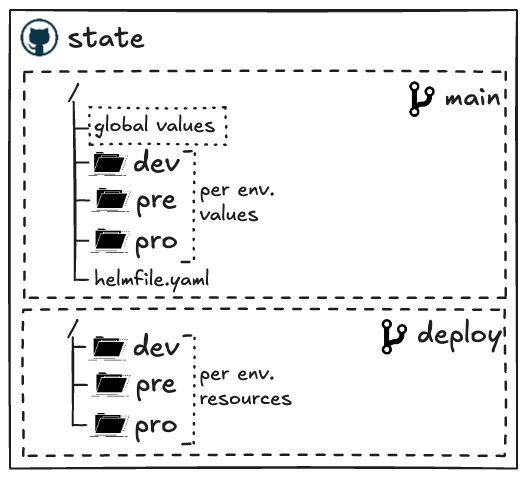
\includegraphics[scale=0.3]{figuras/state}
        \caption{Estructura del repositorio de estado.}
    \end{figure}
\end{frame}

\begin{frame}
    \frametitle{GitOps \& ArgoCD}
    \begin{figure}
        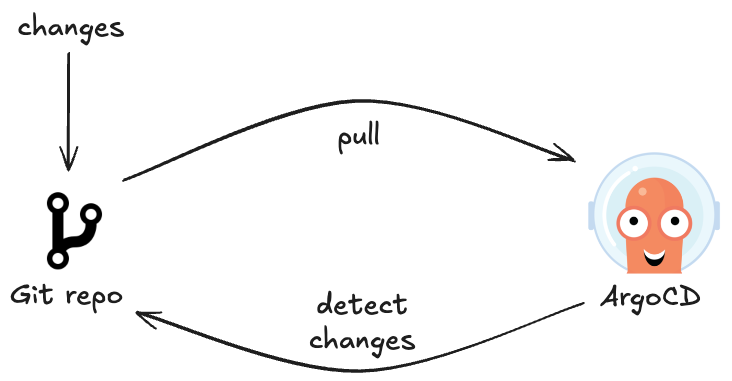
\includegraphics[scale=0.35]{figuras/argocd-simple}
        \caption{Funcionamiento de ArgoCD con GitOps.}
    \end{figure}
\end{frame}

\subsection{CD con Dagger}
\begin{frame}
    \frametitle{Tengo que explicar CD}
\end{frame}

\section{Conclusiones}
\begin{frame}
    \frametitle{Conclusiones}
\end{frame}

% \section{Bibliografía}
% \begin{frame}
%     \frametitle{Bibliografía}
%     \begin{thebibliography}{99}
%         \scriptsize
%         \bibitem{gitlab_architecture} GitLab Inc. ``GitLab Architecture Overview | GitLab Docs.'' Gitlab.com, 2025, {\it https://docs.gitlab.com/development/architecture/\#simplified-component-overview}. Accedido el 26 de agosto del 2025.
%         \bibitem{gitlab_repo} GitLab Inc. ``GitLab.org / GitLab.'' GitLab, 8 Feb. 2020, {\it https://gitlab.com/gitlab-org/gitlab}.
%         \bibitem{gitlab_ci} GitLab Inc. ``Doc/Development/Cicd/\_index.md · Master · GitLab.org / GitLab · GitLab.'' GitLab, 2025, {\it https://gitlab.com/gitlab-org/gitlab/-/blob/master/doc/development/cicd/\_index.md}. Accedido el 26 de agosto del 2025.
%     \end{thebibliography}
% \end{frame}

\end{document}
% Dagger functions (encadenamiento)
% Daggerverse

% \section{Sección 1}
% \subsection{Ejemplo de subsección}
% \begin{frame}
%     \frametitle{Título del frame 1}
%     Cada pantalla tiene su título.
% \end{frame}
%
% \subsection{Ejemplo de lista}
%
% \begin{frame}
%     \frametitle{Lista no numerada}
%     \begin{itemize}
%         \item una
%         \item dos
%         \item tres
%         \item cuatro
%     \end{itemize}
% \end{frame}
%
% \begin{frame}
%     \frametitle{Lista con pausa}
%     \begin{itemize}
%         \item número uno \pause
%         \item número dos \pause
%         \item número tres \pause
%         \item número cuatro
%     \end{itemize}
% \end{frame}
%
% \subsection{Otro ejemplo de lista}
% \begin{frame}
%     \frametitle{Lista numerada}
%     \begin{enumerate}
%         \item una
%         \item dos
%         \item tres
%         \item cuatro
%     \end{enumerate}
% \end{frame}
%
% \section{Sección 2}
% \subsection{Tablas}
%
% \begin{frame}
%     \frametitle{Tablas}
%     \begin{tabular}{|c|l|r|} \hline
%         \textbf{Centrado} & \textbf{Izquierda} & \textbf{Derecha} \\ \hline
%         AAAA              & 1000               & aaaa             \\ \hline
%         BB                & 20                 & bb               \\ \hline
%     \end{tabular}
% \end{frame}
%
% \begin{frame}
%     \frametitle{Tabla con pausa}
%     \begin{tabular}{c c c}
%         A & B & C \\ \pause
%         1 & 2 & 3 \\  \pause
%         A & B & C \\
%     \end{tabular}
% \end{frame}
%
% \section{Sección 3}
% \subsection{Bloques}
%
% \begin{frame}
%     \frametitle{Bloques}
%
%     \begin{block}{Bloque normal}
%         Texto del bloque normal
%     \end{block}
%
%     \begin{exampleblock}{Bloque de ejemplo}
%         Texto del bloque ejemplo
%     \end{exampleblock}
%
%     \begin{alertblock}{Bloque de alerta}
%         Texto del bloque alerta
%     \end{alertblock}
% \end{frame}
%
% \section{Sección 4}
% \subsection{Pantalla dividida}
%
% \begin{frame}
%     \frametitle{Pantalla dividida}
%     \begin{columns}
%         \begin{column}{5cm}
%             \begin{itemize}
%                 \item una lista
%                 \item de puntos
%                 \item mas una tabla
%             \end{itemize}
%         \end{column}
%         \begin{column}{5cm}
%             \begin{tabular}{|c|c|c|} \hline
%                 \textbf{Mes} & \textbf{Día} & \textbf{Hora} \\ \hline
%                 Enero        & 10           & 15:30         \\ \hline
%                 Febrero      & 20           & 20:00         \\ \hline
%             \end{tabular}
%         \end{column}
%     \end{columns}
% \end{frame}
%
% \subsection{Figuras}
% \begin{frame}
%     \frametitle{Incluir figuras}
%     \begin{figure}
%         
\includegraphics[scale=0.3]{figuras/logo_usc.eps}
%         \caption{Logo de la USC}
%     \end{figure}
% \end{frame}
%
% \subsection{Listas con figuras y pausas}
%
% \begin{frame}
%     \frametitle{Listas con figuras y pausas}
%     \begin{columns}
%         \begin{column}{4cm}
%             \begin{itemize}
%                 \item<1-> Una
%                 \item<3-> Dos
%                 \item<5-> Tres
%             \end{itemize}
%             \vspace{3cm}
%         \end{column}
%         \begin{column}{4cm}
%             \begin{overprint}
%                 \includegraphics<2>[scale=0.05]{figuras/logo_usc.eps}
%                 \includegraphics<4>[scale=0.10]{figuras/logo_usc.eps}
%                 \includegraphics<6>[scale=0.15]{figuras/logo_usc.eps}
%             \end{overprint}
%         \end{column}
%     \end{columns}
% \end{frame}
%
% \subsection{Cuando se necesita más espacio}
% \begin{frame}[plain]
%     \frametitle{Pantalla plana con sólo una figura}
%     \begin{figure}
%         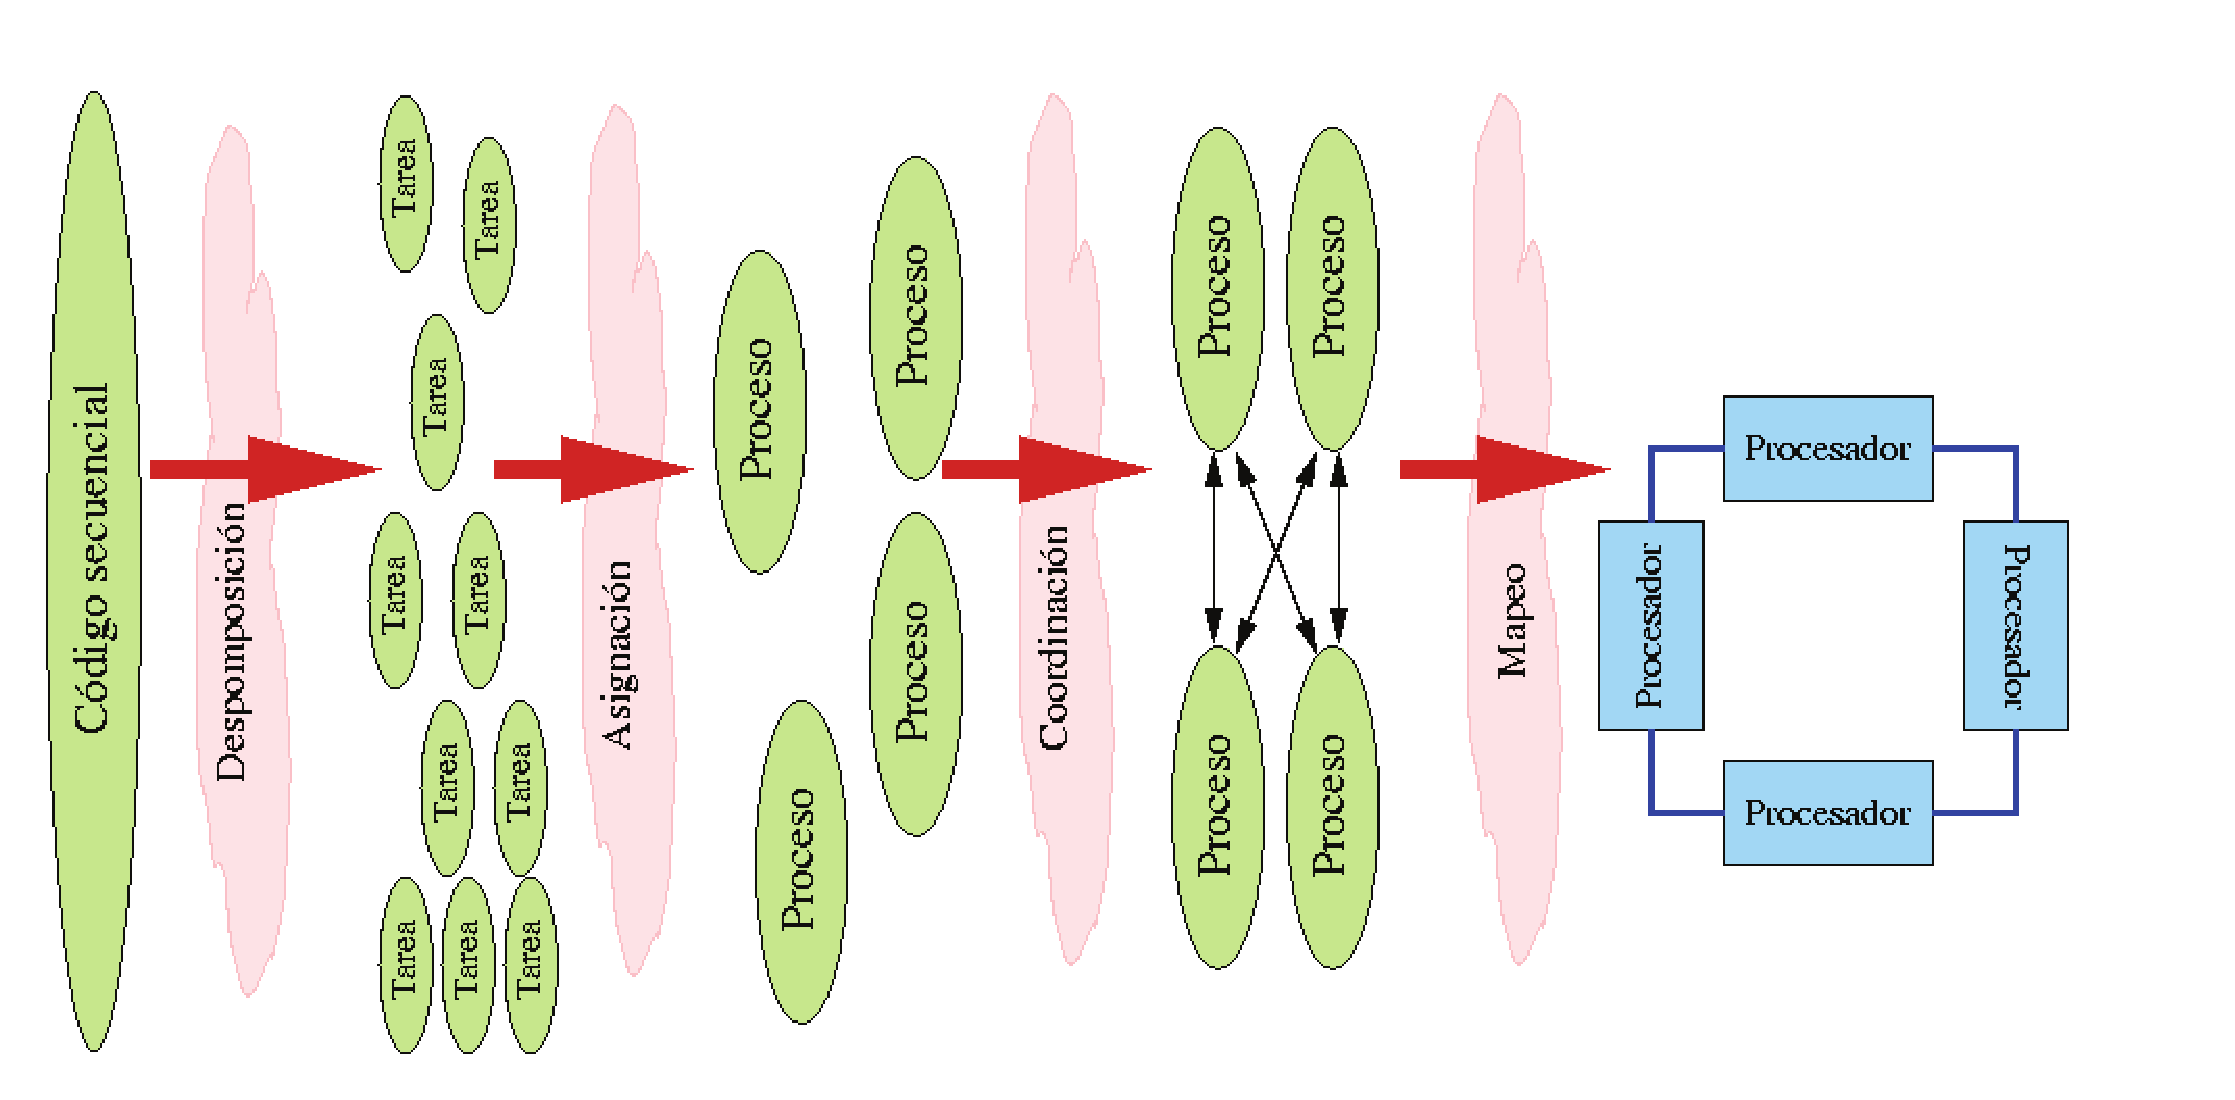
\includegraphics[scale=0.3]{figuras/figura01.eps}
%         \caption{Una figura grande}
%     \end{figure}
% \end{frame}
